\chapter{Модель гистерезисного микроансамбля} \label{chapter:neuron}

В данной главе даётся формальное определение модели нейрона в виде системы обыкновенных дифференциальных уравнений, а так же определяется понятие микроансамбля --- сильно связного объединения нейронов. Анализируются точки равновесия, проводится бифуркационный анализ, а так же моделируются различные сценарии функционирования простейшей модели микроансамбля, в результате чего определяются её характерные свойства. При этом рассматривается применение двух различных функций активации: оригинальной и сигмоидальной. 

Кроме того, для апробации предлагаемой модели микроансамбля на её основе реализуются две нейронных сети, первая из которых решает задачу анализа независимых компонент, а вторая моделирует детерминированный конечный автомат. 


%==============================================================================
%                          Формальное определение модели
%==============================================================================
\section{Формальное определение} \label{section:neuron_model}

Основой для анализируемой в данной главе модели нейрона послужила монография~\cite{EmelyanovYaroslavsky1990}, в которой рассматривается подход к построению искусственной \acr{NN}, потенциально обладающей интеллектуальными свойствами и названной автором \textit{индуктивным автоматом}. Особенность работы заключается в том, что автор предлагает оригинальную модель нейрона и показывает через численные и умозрительные эксперименты, что благодаря ряду локальных свойств совокупность нейронов способна демонстрировать нетривиальное поведение. Однако предложенная нейросетевая модель носит ярко выраженный незаконченный характер и кроме того, преследует целью биологическую правдоподобность, что так же отразилось на сложности модели.

Данная диссертационная работа направлена на потенциальную прикладную значимость модели, в частности, при решении задачи контекстно-зависимого распознавания образов. Поэтому предложенный в работе~\cite{EmelyanovYaroslavsky1990} подход был в значительной мере переосмыслен и в результате была выработана собственная нейросетевая модель: она не содержит биологически обоснованных и стохастических элементов, а так же в противоположность \textit{Integrate-And-Fire} типу модели, где подразумевается моделирование на уровне отдельных импульсов нейрона с частотно-фазовым кодированием информации, является более классической \textit{Firing-Rate}  моделью~\cite{Dayan2001}, в которой выходным параметром нейрона является \socalled частота --- усреднённая по времени частота генерации импульсов. И хотя первый тип обладает более разнообразной поведенческой динамикой и информационной ёмкостью, их практическое применение сопряжено с рядом проблем~[\todo{ссылка?}]. Так же присутствует и ряд других изменений, однако полезные в решении нашей задачи идеи были сохранены.

Таким образом, формальная модель нейрона приобрела следующий вид:
\begin{equation}
	\label{eq:full_single_neuron_model}
    \begin{cases}
	    d\scalar{u}/d\scalar{t} &= \vector{w}^{\top} \vector{x} - \scalar{p} - \mu \scalar{u}, \\
        \scalar{y}              &= f\left( \scalar{u}, \theta \right), \\
    \end{cases}
\end{equation}
где $\scalar{u} \in \specialset{R}$ --- потенциал нейрона, $\vector{x} \in \specialset{R}^{M}$ -- входной вектор нейрона (входной сигнал), $\vector{w} \in \specialset{R}^{M}$ --- вектор весовых коэффициентов нейрона,  $\scalar{p}$ --- внутренний порог нейрона, $\mu \in \left(0;1\right)$ --- константа, характеризующая скорость убывания потенциала нейрона, $\scalar{y} \in \left[0;1\right]$ --- частота нейрона (выходной сигнал), $\theta$ --- управляющий параметр сети, который будет рассмотрен более подробно в следующих главах. 

Для удобства дальнейшего изложения мы применим приём, который часто используется в области нейросетевого моделирования, а именно: положим, что $\vectoritem{x}{0}$ в любой момент времени равно $1$ и $\vectoritem{w}{0}$ равно $-\scalar{p}$, тогда выражением~\eqref{eq:full_single_neuron_model} можно записать в более компактной эквивалентной форме:
\begin{equation}
    \label{eq:single_neuron_model}
    \begin{cases}
    d\scalar{u}/d\scalar{t} &= \vector{w}^{\top} \vector{x} - \mu \scalar{u}, \\
    \scalar{y}              &= f\left( \scalar{u}, \theta \right), \\
    \end{cases}
\end{equation}
которая будет использована далее наравне с выражением~\eqref{eq:full_single_neuron_model}.

Функция активации $f: \specialset{R} \to \left[0;1\right]$ преобразует потенциал нейрона $\scalar{u}$ в его выходную частоту $\scalar{y}$ в виде:
\begin{equation}
    \label{eq:activation_function}
    f\left( \scalar{u}, \theta \right) = g\left( \tilde{\scalar{u}} \right), 
\end{equation}
где $\tilde{\scalar{u}} = \scalar{u} / \theta$, а в качестве $g$ в главе будут рассмотрены две функции, изображённые \onfigure~\ref{fig:model_activation_functions} (далее функции $f$ и $g$ будут в равной степени называться функциями активации):
\begin{itemize}
	\item \textit{Оригинальная} функция $g_{s}$, полученная на основе функции динамического порога $\text{П}^\text{Д}$ из работы~\cite{EmelyanovYaroslavsky1990}, но отличающаяся от неё в виду того, что аргументом функции  $\text{П}^\text{Д}$ является межимпульсный интервал и, что важнее, она не была задана автором аналитически (подробнее вывод функции $g_{s}$ рассмотрен \inappendix~\ref{appendix:activation_function}):
		\begin{equation}
            \label{eq:activation_function_original}
            g_{s}(\tilde{\scalar{u}}) = 
            \begin{cases}
                0                                                                                               &, \tilde{\scalar{u}} < u_{01} \\
                0,1935 + \dfrac{1}{120} \ln\left( \dfrac{\tilde{\scalar{u}}}{2,6 - \tilde{\scalar{u}}} \right)  &, u_{01} \le \tilde{\scalar{u}} \le u_{12} \\
                1 - \dfrac{0,35}{\tilde{\scalar{u}} - k_{12}}                                                   &, \tilde{\scalar{u}} > u_{12} \\
            \end{cases}
		\end{equation}
        где значения коэффициентов равны:
        \begin{align*}
            &z_{12} = 177,84 \cdot \sigma\left(6,18\right) \cdot \left(1 - \sigma\left(6,18\right)\right) \approx 0,37, \\
            &k_{12} = 2,6 \cdot \sigma\left(6,18\right) - z_{12} / 0,755 \approx 2,11, \\
            &u_{01} = 2,6 \cdot \sigma\left(-23,22\right) \approx 0, \\
            &u_{12} = 2,6 \cdot \sigma\left(6,18\right) \approx 2,6,
        \end{align*}
        где $\sigma$ --- логистическая функция.
	\item \textit{Сигмоидальная} функция $g_{\sigma}$, которая получила широкое распространение в области нейронных сетей, нечёткой логики и \other, в виде:
		\begin{equation}
            \label{eq:activation_function_sigma}
			g_{\sigma}(\tilde{\scalar{u}}) = \dfrac{1}{1 + e^{\displaystyle -(\tilde{\scalar{u}} - 3)}}.
		\end{equation}
\end{itemize}

\IncludeFigure{model_activation_functions}{Вид оригинальной $g_{s}$ и сигмоидальной $g_{\sigma}$ функций активации.}

\begin{Definition*}
    Определим \textit{микроансамбль} в виде математической структуры $A = \left\{ \customset{N}, \matrix{V} \right\}$, где $\customset{N} = \left\{ n_{i} \right\}_{i=1}^{N} $ --- множество нейронов, составляющих микроансамбль, и $\matrix{V}_{N \times N}$ --- матрица, задающая топологию и коэффициенты связей между нейронами микроансамбля. При этом размер множества $\customset{N}$ и значение матрицы $\matrix{V}$ фиксированы, \ie не меняются в процессе обучения и функционирования сети, и выбираются заранее, исходя из требуемых вычислительных свойств микроансамбля как целостной вычислительной единицы \acr{NN}.
\end{Definition*}

Основываясь на выражении~\eqref{eq:single_neuron_model}, динамика микроансамбля может быть описана следующим образом:
\begin{equation}
    \label{eq:microensemble_model}
    \begin{cases}
        d\vector{u}/d\scalar{t} &= \matrix{V}^{\top} \vector{y} + \matrix{W}^{\top} \vector{x} - \mu \vector{u}, \\
        \vector{y}              &= f\left( \vector{u}, \theta \right), \\
    \end{cases}
\end{equation}
где все параметры и переменные имеют тот же смысл, что и в выражении~\eqref{eq:single_neuron_model}, но записанные в векторной форме, включая матрицу $\matrix{W}_{M \times N} = \left[ \vector{w}_{1} \ldots \vector{w}_{N} \right]$, составленную из векторов-столбцов $\vector{w}_{i}$ и отражающую связи входного вектора $\vector{x}$ со всеми нейронами микроансамбля.

Для дальнейшего анализа характерных свойств микроансамбля и построения простых нейросетевых моделей необходимо ввести понятие простого микроансамбля.
\begin{Definition*}
    Будем называть микроансамбль $A$ \textit{простым микроансамблем}, если выполнены следующие условия:
    \begin{itemize}
        \item все нейроны микроансамбля соединены друг с другом связями весом $\omega$, \ie: $\matrix{V}_{N\!\times\!N} = \omega \cdot \left( \matrix{J}_{N\!\times\!N} - \matrix{I}_{N} \right)$, где матрицы $\matrix{J}$ и $\matrix{I}$  --- матрица единиц и единичная матрица соответственно;
        \item все нейроны микроансамбля имеют одинаковые связи с входным вектором $\vector{x}$, \ie: $\forall\ i \in \overline{1,N}\ \vector{w}_{i} = \vector{w}$;
        \item начальные условия для всех нейронов микроансамбля совпадают, \ie: \par $\vector{u}|_{t=0} = \scalar{u}^{0} \cdot \matrix{J}_{N\!\times\!1}$, где $\scalar{u}^{0}$ --- начальное значение потенциала нейронов.
    \end{itemize}
\end{Definition*}

В этом случае можно говорить об эквивалентности всех нейронов микроансамбля, а значит всё множество нейронов $\customset{N}$ может быть представленно в виде одного гипер-нейрона с рекуррентной связью на себя, как показано \onfigure~\ref{fig:model_simple_microensemble}. Выражение~\eqref{eq:microensemble_model} при этом примет более простую форму:
\begin{equation}
    \label{eq:simple_microensemble_model}
    \begin{cases}
    d\scalar{u}/d\scalar{t} &= \alpha \scalar{y} + \vector{w}^{\top} \vector{x} - \mu \scalar{u}, \\
    \scalar{y}              &= f\left( \scalar{u}, \theta \right), \\
    \end{cases}
\end{equation}
где параметр $\alpha = \omega \cdot \left( N - 1 \right)$ --- весовой коэффициент рекуррентной связи, который по смыслу отражает связность нейронов микроансамбля. Выражение~\eqref{eq:simple_microensemble_model} так же можно записать в виде:
\begin{equation}
    \nonumber
    d\scalar{u}/d\scalar{t} = \alpha f\left( \scalar{u}, \theta \right) + \vector{w}^{\top} \vector{x} - \mu \scalar{u},
\end{equation}
которое является одной из форм описания рекуррентных нейронов в нейродинамике. Однако запись в виде системы более удобно в том смысле, что явно содержит выходную переменную $y$.

\IncludeFigure{model_simple_microensemble}{Приведение простого микроансамбля с 3-мя нейронами к виду эквивалентного гипер-нейрона с рекуррентной связью.}

Стоит отметить, что в работе~\cite{Pchelkin2003} исследовалась похожая на систему~\eqref{eq:simple_microensemble_model} модель нейронного ансамбля, которая так же была основана на развитии идей индуктивного автомата~\cite{EmelyanovYaroslavsky1990}. Однако автор, во-первых, не учитывал внешнее влияние на нейроны (слагаемое $\vector{w}^{\top} \vector{x}$), и во-вторых, был сосредоточен на конкретной проблеме, а именно на связи поведения модели с \socalled оптимальной частотой --- основополагающим параметром модели индуктивного автомата, который в явном виде отсутствует в рассматриваемой нами модели.


%==============================================================================
%                       Анализ точек равновесия модели
%==============================================================================
\section{Анализ устойчивости и бифуркационный анализ} \label{section:neuron_equilibrium}

Для удобства дальнейшего анализа введём величину $\scalar{i} = \vector{w}^{\top} \vector{x}$ --- внешнее возбуждение микроансамбля, и обозначим правую часть дифференциального уравнения системы~\eqref{eq:simple_microensemble_model} как:
\begin{equation}
    \label{eq:functional_u}
    F(\scalar{u}) = \alpha f\left( \scalar{u}, \theta \right) + \scalar{i} - \mu \scalar{u}.
\end{equation}
Сразу отметим, что в такой форме записи выходная переменная $y$ присутствует неявно через внутреннюю переменную $u$, поэтому, применив формулу~\eqref{eq:activation_function}, определяющую функцию $f$, данное выражение можно переписать в виде:
\begin{equation}
    \label{eq:functional_y}
    F(\scalar{y}) = \alpha \scalar{y} + \scalar{i} - \mu \theta g^{-1}(\scalar{y}),
\end{equation}
где переменная $y$ присутствует уже явно, а $g^{-1}$ --- обратная функция к $g$. Для определённых нами ранее функций активации обратные будут определяться следующим образом:
\begin{itemize}
    \item Для \textit{оригинальной} функции $g_{s}$, заданной выражением~\eqref{eq:activation_function_original}:
    \begin{equation}
        \label{eq:unactivation_function_original}
        g_{s}^{-1}(\scalar{y}) = 
        \begin{cases}
            \dfrac{2,6}{1 + e^{\displaystyle -120 \cdot (\scalar{y} - 0,1935)}} &, y \in \left[0; y_{12}\right] \\
            k_{12} + \dfrac{0,35}{1 - \scalar{y}}                               &, y \in \left(y_{12}; 1\right] \\
        \end{cases}
    \end{equation}
    где $y_{12} = 1/3,5$.
    \item Для \textit{сигмоидальной} функции $g_{\sigma}$, заданной выражением~\eqref{eq:activation_function_sigma}:
    \begin{equation}
        \label{eq:unactivation_function_sigma}
        g_{\sigma}^{-1}(\scalar{y}) = 3 + \ln\left(\dfrac{\scalar{y}}{1 - \scalar{y}}\right),\;y \in \left[0; 1\right].
    \end{equation}
\end{itemize}

Для нахождения устойчивых точек системы~\eqref{eq:simple_microensemble_model}, описывающей динамику простого микроансамбля, необходимо найти корни уравнения $F(.) = 0$. Однако в виду того, что в обоих выражениях~\eqref{eq:functional_u} и~\eqref{eq:functional_y} переменная одновременно встречается в основании и показателе степени, решить равенство аналитически невозможно. 

Поэтому будем рассматривать решение графически, причём в виде пересечения двух кривых, приравняв выражение~\eqref{eq:functional_y} к нулю и переписав результат в следующем виде:
\begin{equation}
    \label{eq:graphic_solution}
    \scalar{i} = - \alpha \scalar{y} + \mu \theta g^{-1}(\scalar{y}),
\end{equation}
где левая часть выражения отражает внешнее воздействие на микроансамбль, а правая --- внутреннюю динамику микроансамбля. Такая форма решения более удобна по сравнению с непосредственным изображением функции $F(.)$, т.к. позволит сразу же ставить в соответствие внешнему возбуждению $\scalar{i}$, линейно зависящему от входного вектора $\vector{x}$, результирующую выходную частоту $\scalar{y}$.

При этом ещё раз отметим, что параметры $i$ и $\theta$ могут меняться в процессе функционирования сети, а параметры $\alpha$ и $\mu$ подбираются заранее и фиксируются в качестве констант модели.

%==============================================================================
\subsection{Анализ модели с сигмоидальной функцией активации}

Сперва рассмотрим более простой вариант с \textit{сигмоидальной} функцией активации. Как будет доказано в дальнейшем, в этом случае система~\eqref{eq:simple_microensemble_model} обладает двумя качественно разными режимами функционирования, для которых \onfigure~\ref{fig:analysis_sigm_equilibriums} изображены графические решения согласно выражению~\eqref{eq:graphic_solution} и соответствующие графики функции $F(\scalar{y})$:
\begin{itemize}
    \item[а)] система имеет ровно одну точку устойчивого равновесия (точка $\scalar{y}^{*}$) и её положение зависит исключительно от параметров системы, \ie между внешним возбуждением $\scalar{i}$ и частотой нейрона $\scalar{y}$ существует нелинейное, но взаимооднозначное соответствие (использованные значения параметров: $i = 3$, $p = 1,25$, $\mu = 0,75$, $\alpha = 1,0$ и $\theta = 1$);
    \item[б)] система может иметь одну или две точки устойчивого равновесия (точки $\scalar{y}_{1,2}^{*}$), причём во втором случае без знания текущего состояния системы невозможно предсказать выходную частоту $\scalar{y}$ по внешнему возбуждению $\scalar{i}$ (использованные значения параметров: $i = 1$, $p = 1,25$, $\mu = 0,75$, $\alpha = 5,0$ и $\theta = 1$).
\end{itemize}

%Сперва рассмотрим более простой вариант с \textit{сигмоидальной} функцией активации. Как будет показано в дальнейшем, в этом случае система~\eqref{eq:simple_microensemble_model} обладает двумя качественно разными режимами функционирования, поэтому \onfigure~\ref{fig:analysis_sigm_equilibriums} для обоих из них изображены графические решения согласно выражению~\eqref{eq:graphic_solution}:
%\begin{itemize}
%    \item[а)] в модели возможно существование только одной точки устойчивого равновесия $\scalar{y}^{*}$ и её положение зависит исключительно от значений параметров системы, \ie с функциональной точки зрения модель производит нелинейное преобразование внешнего возбуждения $\scalar{i}$ в частоту $\scalar{y}$;
%    \item[б)] в модели возможно существование только одной точки устойчивого равновесия 
%\end{itemize}

%В этом случае система~\eqref{eq:simple_microensemble_model} может находиться в двух качественно разных режимах, что в дальнейшем будет показано аналитически. Поэтому \onfigure~\ref{fig:analysis_sigm_equilibriums} графически изображены решения для обоих случаев: а) в системе существует только одна точка равновесия $\scalar{y}^{*}$ и её положение напрямую зависит от значения параметра $\scalar{i}$; б) в системе возможно существование от одной до трёх точек равновесия $\scalar{y}^{*}_{1,2,3}$ и решение в некоторых случаях зависит не только от значения параметра $\scalar{i}$, но и от начальных условий.

%При использовании \textit{сигмоидальной} функции активации система~\eqref{eq:simple_microensemble_model} может находиться в двух качественно разных режимах, что изображено графически \onfigure~\ref{fig:analysis_sigm_equilibriums} и в дальнейшем будет показано аналитически. В первом случае (\seefigure~\ref{fig:analysis_sigm_equilibriums}а: $\mu = 0,75$, $\alpha = 1,0$ и $\theta = 1,0$) 

%В дальнейшем  и зависит от значений параметров $\mu$, $\alpha$ и $\theta$ 

\IncludeFigure{analysis_sigm_equilibriums}{Анализ устойчивости особых точек.}

\newpage
\IncludeFigure{analysis_sigm_stability}{Анализ устойчивости особых точек.}
\IncludeFigure{analysis_sigm_bifurcations}{Бифуркационные диаграммы.}
\IncludeFigure{analysis_sigm_solution_surface}{Бифуркационные диаграммы.}

\newpage
\IncludeFigure{model_sigm_configurations}{Конфигурации решения в различных точках плоскости параметров.}


%==============================================================================
\subsection{Анализ модели с оригинальной функцией активации}


%==============================================================================
%                       Характерные параметры модели
%==============================================================================
\section{Характерные свойства и динамика} \label{section:neuron_dynamic}

Для выполнения численных экспериментов с рабочей моделью необходимо в первую очередь привести её к эквивалентной дискретной форме, применив один из разностных методов. Для этого в ходе исследований было рассмотрено применение классических методов, таких как явный метод Эйлера, модифицированный метод Эйлера с пересчётом (разновидность метода Рунге-Кутты второго порядка точности), а так же явный метод Рунге-Кутты четвёртого порядка точности~\cite{Hairer1990}. Более подробно этот вопрос освещён \inappendix~\ref{appendix:differential_schemes_compare}. Здесь же отметим, что при выборе разумного с точки зрения точности и вычислительной эффективности шага $h$ использование того или иного метода не вносило существенных изменений в результаты численных экспериментов. Поэтому описанные далее в главе результаты подразумевают применение явного метода Эйлера с шагом $h = 0,01$:
\begin{equation*}
    \begin{cases}
        \scalar{u^{t+1}} = \scalar{u^{t}} + h \times ( \alpha\scalar{y^{t}} + \scalar{i^{t}} - \scalar{p^{t}} - \mu\scalar{u^{t}} ), \\ 
        \scalar{y^{t+1}} = f(\scalar{u^{t+1}}, \theta).
    \end{cases}
\end{equation*}


%==============================================================================
\subsection{Динамика модели с сигмоидальной функцией активации}

%==============================================================================
\subsection{Динамика модели с оригинальной функцией активации}

%==============================================================================
\subsection{Характерные свойства модели}


%==============================================================================
%               Моделирование простейшей нейронной сети
%==============================================================================
\section{Моделирование простейших нейронных структур} \label{section:neuron_modeling}

Для проверки принципиальной работоспособности предлагаемой модели далее будут рассмотрены две задачи: задача анализа независимых компонент (\acr{ICA}) и задача построения нейросетевого детерминированного конечного автомата (\acr{FSM}). Для их решения будут смоделированы простые нейронные сети с применением микроансамблей в качестве элементарных элементов. При этом для решения первой задачи параметры модели будут соответствовать <<мягкому>> режиму работы, чтобы продемонстрировать\todo{...}  При решении второй задачи параметры модели будут соответствовать <<жёсткому>> режиму, демонстрируя\todo{...}

\todo{Может быть в этой главе оставить ICA, а FSM перенести в следующую?.. скорее нет, чем да...}

%==============================================================================
\subsection{Решение задачи анализа независимых компонент}

Задача анализа независимых компонент, более подробная постановка которой изложена в Приложении~\ref{appendix:ica_description}, имеет важное прикладное значение, будучи связанной с решением таких проблем, как слепое разделение сигналов и снижение размерности данных~\cite{Hyvarinen2004}. Мы рассмотрим решение частной задачи \acr{ICA} --- <<F{\"o}ldiak bars>>~\cite{Foldiak1990}, которая часто используется в нейросетевой области для первичной проверки соответствующих моделей.

Входные данные представляют собой бинарные изображения размером $8\,\times\,8$ пикселей, сгенерированные с использованием 16-ти независимых компонент: 8-ми горизонтальных и 8-ми вертикальных линий, каждая из которых появлятся на изображении с вероятностью $1/8$ --- независимые компоненты и примеры получаемых на их основе изображений представлены \onfigure~\ref{img:ica_patterns}. Решение же задачи заключается, во-первых, в нахождении в процессе обучения независимых компонент, использованных при генерации изображений, и во-вторых, в разложении в процессе штатной работы входных данных по найденным независимым компонентам. Другими словами, в результате обучения каждой независимой компоненте необходимо поставить в соответствие некоторый нейрон, активность которого будет отражать наличие этой компоненты во входном изображении.

\begin{figure}[ht]
    \makebox[\textwidth][c]{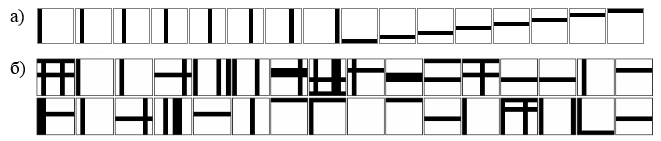
\includegraphics[width=1.0\textwidth]{ica_patterns}}
    \caption{Бинарные изображения размером 8х8 пикселей: а) набор из 16-ти независимых компонент; б) примеры входных паттернов.}
    \label{img:ica_patterns}
\end{figure}

Стоит отметить, что данная постановка задачи соответствует классу нелинейных задач, т.к. в точках пересечения горизонтальных и вертикальных линий происходит не обычная операция сложения значений $(x + y)$, а сложение значений по модулю: $(x + y) \bmod 1$ ---, что вносит нелинейные искажения в складываемые изображения линий.

\subsubsection{Модель нейронной сети}

Для решения данной задачи была реализована однослойная нейронная сеть, состоящая из 16-ти нейронов, что отражает наши априорные знания о числе ожидаемых независимых компонент в обрабатываемых данных. Формальная модель \acr{NN} имеет вид:
\begin{equation}
    \nonumber
    \begin{cases}
        \dot{\vector{u}} &= \left(\alpha \matrix{I} - \matrix{V} \right)^{\top} \vector{y} + \matrix{W}^{\top} \vector{x} - \mu \vector{u},\\
        \vector{y}       &= f(\vector{u}),
    \end{cases}
\end{equation}
где $\vector{x}_{64 \times 1}$ --- входной вектор, представляющий собой линеаризованное по столбцам входное изображение, $\matrix{W}_{64 \times 16}$ --- как и ранее, матрица, отражающая возбуждающие связи от входного вектора к элементами сети, $\matrix{V}_{16 \times 16}$ --- матрица, отражающая тормозные связи между самими элементами сети. В соответствии с работой~\cite{Fyfe2007}, использование взаимных тормозных связей, обучаемых хэббо-подобным правилом, будет приводить к взаимной декорреляции выходов \acr{NN}. В качестве активационной функции была применена оригинальная функция $s$ (ХХХ) и использованы следующие значения параметров: $\mu = 0,75$, $\theta = 1$, $\alpha = (N - 1) \cdot \omega = 10 \cdot 0,25 = 2,5$ и $p = 1,01$.

Для обучения как возбуждающих, так и тормозных связей использовался один из вариантов STDP-правила~\cite{Izhikevich2003} (\todo{ЗАМЕНИТЬ НА ОБЫЧНОЕ ХЭББОВСКОЕ ПРАВИЛО}):
\begin{equation}
    \nonumber
    \begin{cases}
        \Delta_{ji} &= 
        \begin{cases}
            \vector{y}_{j} \vector{y}_{i} \left( \dfrac{A_{E}}{1/\tau_{E} + \vector{y}_{i}} + \dfrac{A_{I}}{1/\tau_{I} + \vector{y}_{i}}\right), &\text{ если } i \ne j \\
            0, &\text{ иначе } \\
        \end{cases} \\
        \vector{w}_{ji} &= \max \left( 0, \vector{w}_{ji} + \beta_{\vector{w}} \Delta_{ji} \right), \\
        \vector{v}_{ji} &= \max \left( 0, \vector{v}_{ji} - \beta_{\vector{v}} \Delta_{ji} \right), \\
    \end{cases}
\end{equation}
где $A_{E} = 1,01$, $A_{I} = -0,58$, $\tau_{E} = 5$, $\tau_{I} = 38$, $\beta_{\vector{w}} = 0,001$, $\beta_{\vector{v}} = 0,01$, а функция $\max$ обеспечивает неотрицательность элементов матриц $\matrix{W}$ и $\matrix{V}$. Кроме того, после каждой итерации выполнялась нормализация весовых матриц по столбцам, так чтобы $\forall i\ \sum_{j}\vector{w}_{ji} = w^{total}$, где $w^{total} = 2,7$, и $\forall i\ \sum_{j}\vector{v}_{ji} = v^{total}$, где $v^{total} = 5,4$.

\subsubsection{Результаты численных экспериментов}

\begin{figure}[ht]
    \makebox[\textwidth][c]{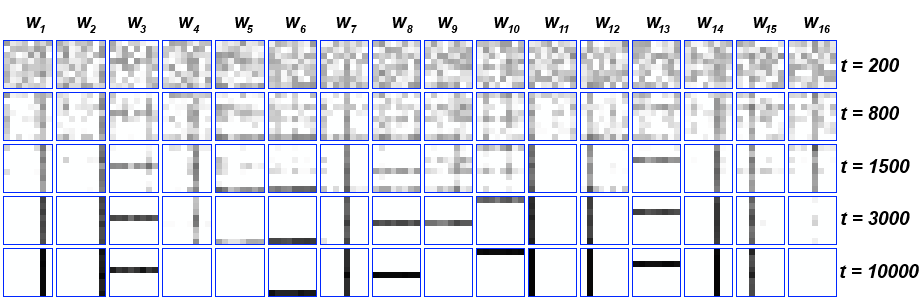
\includegraphics[width=1.0\textwidth]{ica_learning_weights}}
    \caption{\todo{Изменение векторов-столбцов возбуждающей матрицы $\matrix{W}$ в процессе обучения...}}
    \label{img:ica_learning_weights}
\end{figure}

\begin{figure}[ht]
    \makebox[\textwidth][c]{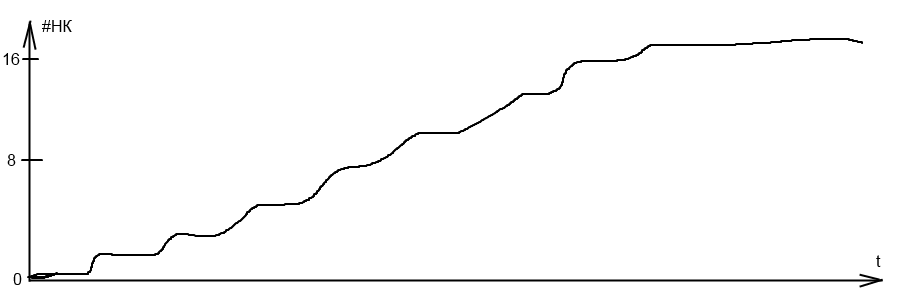
\includegraphics[width=1.0\textwidth]{ica_learning_progress}}
    \caption{\todo{Количество найденных уникальных компонент в процессе обучения...}}
    \label{img:ica_learning_progress}
\end{figure}

\begin{figure}[ht]
    \makebox[\textwidth][c]{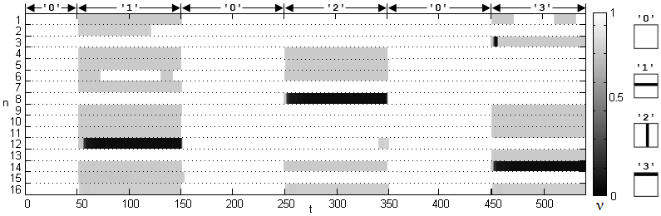
\includegraphics[width=1.0\textwidth]{ica_modeling_result}}
    \caption{\todo{Результат моделирования...}}
    \label{img:ica_modeling_result}
\end{figure}


%==============================================================================
\subsection{Построение нейросетевого конечного автомата}

\todo{Вводная часть...}

\subsubsection{Модель нейронного конечного автомата}

Определим детерминированный конечный автомат (\acr{FSM})~\cite{Hopcroft2008} как формальную математическую структуру $M = \left( \usualset{A}, \usualset{S}, s_{0}, \delta \right)$, где $\usualset{A}$ --- конечное множество входных символов (входной алфавит), $\usualset{S}$ --- конечное множество состояний автомата, $s_{0} \in \usualset{S}$ --- начальное состояние автомата, $\delta\!: \usualset{S}\!\times\!\usualset{A} \to \usualset{S}$ --- функция перехода, отображающая упорядоченную пару элементов (состояние автомата и входной символ) в новое состояние автомата. Если мы обозначим через $q \in \usualset{S}$ текущее состояние автомата, которое в начальный момент времени совпадает с $s_{0}$, то функционирование автомата заключается в последовательном считывании символов $a_{i}$ из входной последовательности $\left\{ a_{0} a_{1} \ldots | a_{j} \in \usualset{A} \right\}$ и переходе в новое состояние: $q = \delta \left( q, a_{i} \right)$. Стоит отметить, что в структуру $M$ часто добавляют множество \socalled заключительных состояний $\usualset{F} \subseteq \usualset{S}$ для верификации считанной входной последовательности, однако в данной работе в этом нет необходимости.

Построение нейросетевой модели по заданной структуре \acr{FSM} можно разбить на две части: построение топологии сети и подбор весовых коэффициентов связей сети. Для задания топологии в первую очередь необходимо каждому элементу всех множеств структуры $M$ поставить в соответствие свой нейрон $n_{i}$: обозначим множество $\left\{ n_{k} | k = \usualset{A} \right\}$, соответствующее множеству $\usualset{A}$, как множество \inquotes{входных} нейронов, множество $\left\{ n_{k} | k = \usualset{S} \right\}$, соответствующее множеству $\usualset{S}$, как множество нейронов \inquotes{состояний} и множество $\left\{ n_{k} | k = D(\delta) \right\}$, соответствующее множеству $S\!\times\!A$ (исключая элементы, для которых отображение $\delta$ не определено), как множество нейронов \inquotes{переходов}. Таким образом, сеть будет состоять из $N = \left|\usualset{A}\right| + \left|\usualset{S}\right| + \left|D(\delta)\right|$ нейронов.

Далее каждому переходу, заданному как элемент множества $\{ \left( s_{i}, s_{j}, a_{k} \right) | \exists \delta\!: s_{i}\!\times\!a_{k} \to s_{j} \}$, необходимо поставить в соответствие набор связей между нейронами сети. Учтём, что в любой момент времени может считываться только один входной символ и должен быть активен только один нейрон \inquotes{состояния} (исключая периоды смены текущего состояния \acr{FSM}, которые связаны с инертностью системы). Поэтому переход из одного состояния в другое является результатом взаимодействия тех нейронов, которые непосредственно соответствуют данному переходому в структуре $M$, а активность остальных должна быть пренебрежимо мала. В результате такой локализации вычислений нейронные связи в сети можно представить в виде типизированного набора, соответствующего каждому переходу в \acr{FSM}: $\beta_{st}$ --- двунаправленная тормозная связь между $n_{s_{i}}$ и $n_{s_{j}}$, $\beta_{tr}$ --- тормозная связь от $n_{s_{i}\!\times\!a_{k}}$ к $n_{a_{k}}$, $\gamma_{st}$ --- возбуждающая связь от $n_{s_{i}}$ к $n_{s_{i}\!\times\!a_{k}}$, $\gamma_{tr}$ -- возбуждающая связь от $n_{s_{i}\!\times\!a_{k}}$ к $n_{s_{j}}$, $\gamma_{in}$ --- возбуждающая связь от $n_{a_{k}}$ к $n_{s_{i}\!\times\!a_{k}}$. \todo{Таким образом, матрица связей \acr{NN} будет имеет следующий вид: ...}

Значения весовых коэффициентов связей подбираются путём решения системы неравенст, описывающей требуемое от элементов сети поведение. Для произвольного перехода $s_{i}\!\times\!a_{k}~\to~s_{j}$ эти требования можно сформулировать следующим образом:. \todo{Формально это соответствует следующей системе уравнений:}

Данная схема позволяет построить для произволного \acr{FSM} функционально эквивалентную нейросетевую модель. Перед началом моделирования начальное состоние $S_{0}$ может быть задано явно, например, как одно из начальных условий: $\nu_{s_{0}} = \nu^{high}$.

Для наглядности \onfigure~\ref{img:fsm_example_topology}а изображена простейшая схема \acr{FSM} с $\usualset{A} = \{ a_{1}, a_{2} \}$, $\usualset{S} = \{ s_{1}, s_{2}, s_{3} \}$ и функцией $\delta$, определённой как $\{ s_{1}\!\times\!a_{1} \to s_{2}$, $s_{2}\!\times\!a_{1} \to s_{3}$, $s_{3}\!\times\!a_{2} \to s_{1} \}$. Результат применения описанного выше преобразования --- функционально эквивалентная \acr{NN}, изображённая \onfigure~\ref{img:fsm_example_topology}б (на рисунке также изображены рекуррентные связи нейронов $\alpha_{st}$ и $\alpha_{tr}$). Используя параметры сети \todo{параметры}, можно вычислить коэффициенты связей (\seefigure~\ref{img:fsm_example_weights}): \todo{коэффициенты}.

\begin{figure}[ht]
    \makebox[\textwidth][c]{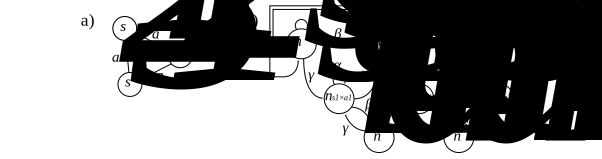
\includegraphics[width=1.0\textwidth]{fsm_example_topology}}
    \caption{Пример построения нейросетевого \acr{FSM}: а) диаграмма состояний автомата; б) эквивалентная диаграмме состояний схема \acr{NN}.} 
    \label{img:fsm_example_topology}  
\end{figure}

\begin{figure}[ht]
    \makebox[\textwidth][c]{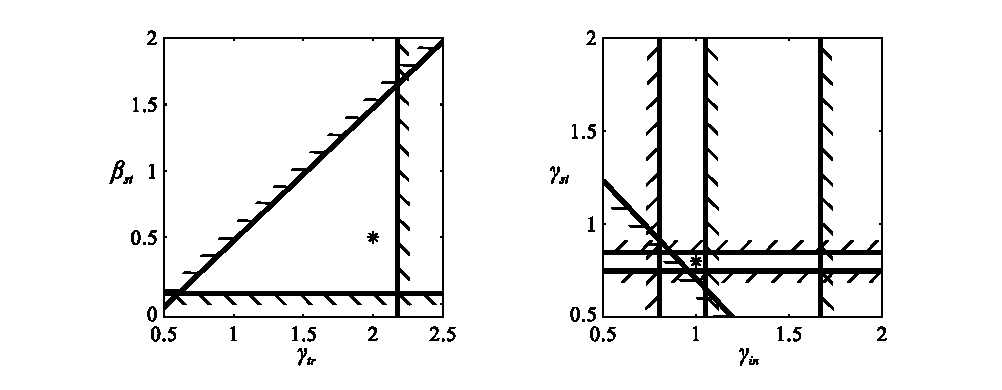
\includegraphics[width=1.2\textwidth]{fsm_example_weights}}
    \caption{Допустимые области значений для весовых коэффициентов, полученные при использовании параметров: \todo{значения параметров}. Ограничения обусловлены функциональными требованиями, наложенными на различные типы нейронов. } 
    \label{img:fsm_example_weights}  
\end{figure}


\subsubsection{Результаты численных экспериментов}

Результат моделирования простейшей схемы \acr{FSM} из предыдущего подраздела (\seefigure~\ref{img:fsm_example_topology}) представлен \onfigure~\ref{img:fsm_example_dynamic}, на котором отражена частота нейронов \inquotes{состояний} и периоды предъявления входных символов. Видно, что при подаче допустимых входных символов, \ie для которых определён переход из текущего состояния, происходит смена конфигурации: соответствующий текущему состоянию нейрон становится неактивным, а соответствующий новому состоянию --- активным. В то же время, при подаче недопустимого символа (интервал времени $[350; 375]$) состояние сети качественно остаётся без изменений. Кроме того, стоит отметить что непрерывное предъявление входного символа приводит к последовательной смене состояний до тех пор, пока схема автомата это допускает (интервал времени $[450; 500]$), что отражает периодичность происходящих в модели процессов.

\begin{figure}[ht]
    \makebox[\textwidth][c]{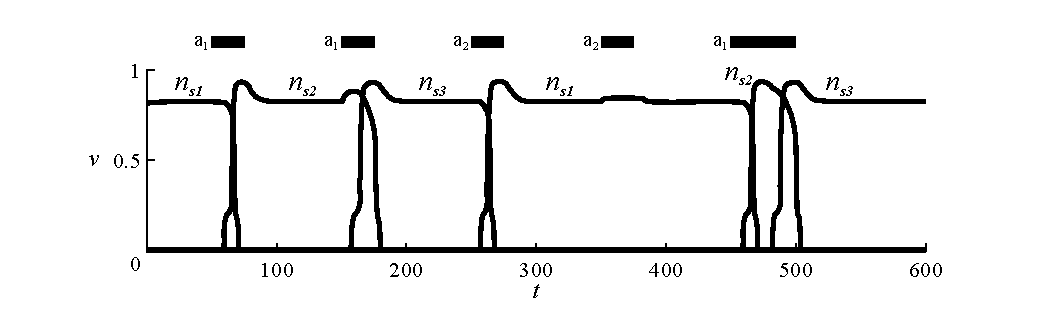
\includegraphics[width=1.1\textwidth]{fsm_example_dynamic}}
    \caption{Динамика нейронов \inquotes{состояний} нейросетевой модели \acr{FSM}, представленной \onfigure~\ref{img:fsm_example_topology}б. Верхние горизонтальные линии отражают временне периоды считывания входных символов.} 
    \label{img:fsm_example_dynamic}  
\end{figure}

Также работоспособность данного подхода проверялась и на более сложных примерах \acr{FSM}, один из которых приведён \onfigure~\ref{img:fsm_model_topology}, --- стоит отметить наличие в диаграмме состояний циклов и двойных переходов (наличие двойных дуг от одного состояния к другому). Как и ранее, в результате применения описанного выше преобразования была получена функционально эквивалентная нейросетевая модель со следующими параметрами: \todo{параметры}. Различные численные эксперименты, один из которых приведён \onfigure~\ref{img:fsm_model_dynamic}, показали, что нейросетевая модель автомата успешно обрабатывает любую последовательность входных символов, игнорируя недопустимые символы. При этом работоспособность сохраняется и при обработке достаточно длинных последовательностей (максимальная использованная длина последовательности составила 1000 символов) и при наличии больших временн\'{ы}х задержек между предъявлениями символов (максимальная использованная задержка составила порядка 10000 единиц), что подтверждает работоспособность данного подхода.

\begin{figure}[ht]
    \makebox[\textwidth][c]{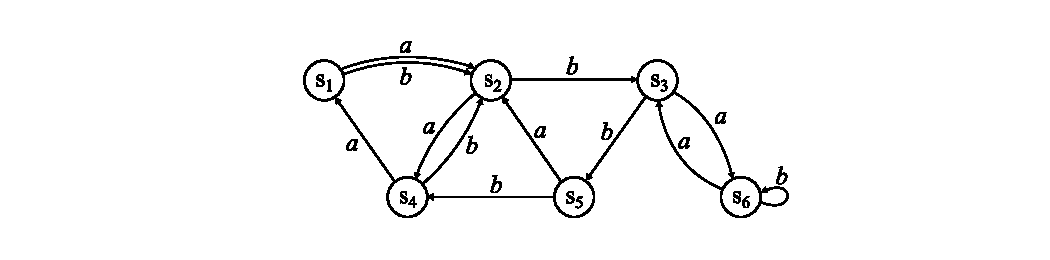
\includegraphics[width=1.2\textwidth]{fsm_model_topology}}
    \caption{Диаграмма состояний \acr{FSM}, использованного в процессе моделирования.}
    \label{img:fsm_model_topology}  
\end{figure}

\begin{figure}[ht]
    \makebox[\textwidth][c]{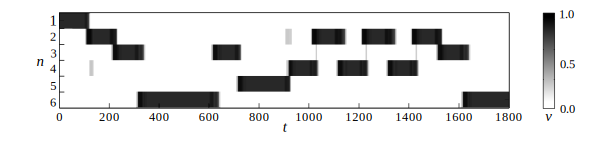
\includegraphics[width=1.1\textwidth]{fsm_model_dynamic}}
    \caption{Результаты численного моделирования нейросетевого \acr{FSM}, представленного \onfigure~\ref{img:fsm_model_topology}. Ось ординат соответствует индексам нейронов \inquotes{состояний}. Значение частоты нейронов выражено оттенками серого в соответствии со шкалой справа.} 
    \label{img:fsm_model_dynamic}  
\end{figure}

%==============================================================================
%                               Выводы по главе
%==============================================================================
\section{Выводы по главе \thechapter} \label{section:neuron_concls}



